%% This is file `elsarticle-template-1-num.tex',
%%
%% Copyright 2009 Elsevier Ltd
%%
%% This file is part of the 'Elsarticle Bundle'.
%% ---------------------------------------------
%%
%% It may be distributed under the conditions of the LaTeX Project Public
%% License, either version 1.2 of this license or (at your option) any
%% later version.  The latest version of this license is in
%%    http://www.latex-project.org/lppl.txt
%% and version 1.2 or later is part of all distributions of LaTeX
%% version 1999/12/01 or later.
%%
%% Template article for Elsevier's document class `elsarticle'
%% with numbered style bibliographic references
%%
%% $Id: elsarticle-template-1-num.tex 149 2009-10-08 05:01:15Z rishi $
%% $URL: http://lenova.river-valley.com/svn/elsbst/trunk/elsarticle-template-1-num.tex $
%%
\documentclass[preprint,12pt]{elsarticle}

%% Use the option review to obtain double line spacing
%% \documentclass[preprint,review,12pt]{elsarticle}

%% Use the options 1p,twocolumn; 3p; 3p,twocolumn; 5p; or 5p,twocolumn
%% for a journal layout:
%% \documentclass[final,1p,times]{elsarticle}
%% \documentclass[final,1p,times,twocolumn]{elsarticle}
%% \documentclass[final,3p,times]{elsarticle}
%% \documentclass[final,3p,times,twocolumn]{elsarticle}
%% \documentclass[final,5p,times]{elsarticle}
%% \documentclass[final,5p,times,twocolumn]{elsarticle}

%% The graphicx package provides the includegraphics command.
\usepackage{graphicx}
\usepackage{hyperref}
%% The amssymb package provides various useful mathematical symbols
\usepackage{amssymb}
%% The amsthm package provides extended theorem environments
%% \usepackage{amsthm}

%% The lineno packages adds line numbers. Start line numbering with
%% \begin{linenumbers}, end it with \end{linenumbers}. Or switch it on
%% for the whole article with \linenumbers after \end{frontmatter}.
\usepackage{lineno}

\usepackage[utf8]{inputenc}
\usepackage{array}
\usepackage{booktabs}
\usepackage{amsmath}

%% natbib.sty is loaded by default. However, natbib options can be
%% provided with \biboptions{...} command. Following options are
%% valid:

%%   round  -  round parentheses are used (default)
%%   square -  square brackets are used   [option]
%%   curly  -  curly braces are used      {option}
%%   angle  -  angle brackets are used    <option>
%%   semicolon  -  multiple citations separated by semi-colon
%%   colon  - same as semicolon, an earlier confusion
%%   comma  -  separated by comma
%%   numbers-  selects numerical citations
%%   super  -  numerical citations as superscripts
%%   sort   -  sorts multiple citations according to order in ref. list
%%   sort&compress   -  like sort, but also compresses numerical citations
%%   compress - compresses without sorting
%%
%% \biboptions{comma,round}

% \biboptions{}

\journal{Scientific Data}

\begin{document}

\begin{frontmatter}

%% Title, authors and addresses

\title{Friends don't let friends over-fit: Benchmarking open-source prediction methods on public building electrical meter data}
%% use the tnoteref command within \title for footnotes;
%% use the tnotetext command for the associated footnote;
%% use the fnref command within \author or \address for footnotes;
%% use the fntext command for the associated footnote;
%% use the corref command within \author for corresponding author footnotes;
%% use the cortext command for the associated footnote;
%% use the ead command for the email address,
%% and the form \ead[url] for the home page:
%%
%% \title{Title\tnoteref{label1}}
%% \tnotetext[label1]{}
%% \author{Name\corref{cor1}\fnref{label2}}
%% \ead{email address}
%% \ead[url]{home page}
%% \fntext[label2]{}
%% \cortext[cor1]{}
%% \address{Address\fnref{label3}}
%% \fntext[label3]{}


%% use optional labels to link authors explicitly to addresses:
%% \author[label1,label2]{<author name>}
%% \address[label1]{<address>}
%% \address[label2]{<address>}

% \author{Clayton Miller}
% \cortext[cor1]{Corresponding author email: clayton@nus.edu.sg, Phone: +65 81602452}

\address{Building and Urban Data Science (BUDS) Lab, Dept. of Building, School of Design and Environment (SDE), National University of Singapore (NUS)}
% Building and Urban Data Science (BUDS) Group, 
% \address[label1]{ETH Z\"urich, Institute of Technology in Architecture (ITA), Architecture and Building Systems (A/S), Z\"urich, Switzerland}
% \address[label2]{Future Cities Laboratory (FCL), Singapore-ETH Center (SEC), Singapore}
% \address[label3]{Andlinger Center for Energy and the Environment, School of Architecture, Princeton University, Princeton, NJ, USA}
% \address{*Corresponding author: Phone: +1-402-403-0090, miller.clayton@arch.ethz.ch}

\begin{abstract}
%% Text of abstract
Prediction is a common machine learning (ML) technique used on building energy consumption data. This process is valuable for anomaly detection, load profile-based control, energy plant systems optimizations, and measurement and verification procedures. Literally hundreds of building energy prediction techniques have been developed over the last three decades, yet there is still no consensus on which techniques are the most effective for various building types. In addition, many of the techniques developed are proprietary and unavailable to the general research community. This paper outlines a library of open source regression techniques from the \emph{Scikit-Learn} Python library and describes the process of applying them to open hourly electrical meter data from 482 non-residential buildings from data from the \emph{Building Data Genome Project}. The results illustrate that there is no \emph{one size-fits-all} modeling solution and that various types of temporal behavior are difficult to capture using machine learning. This framework and methodology is designed to be a \emph{baseline} implementation for other building energy data prediction methods developed by commercial providers or the wider research community. The benchmark data set can also be expanded with numerous other building performance data from a wider representation of buildings from around the world. The entire code base and data sets are found openly in a Github repository. The use of a baseline data set in future prediction research results in comparability and reproducibility of techniques in the built environment domain. 

% , the \emph{M\&V 2.0} R package and the \emph{eemeter} Python package
% non time-series machine learning models and can be further applied using other building industry-specific and time-series forecasting models.
\end{abstract}

\begin{keyword}
Building energy prediction \sep Building performance prediction \sep Performance prediction \sep Machine learning \sep Smart meters \sep Artificial neural networks \sep Support vector machines \sep Deep Learning
\end{keyword}

\end{frontmatter}
\linenumbers

\section{Introduction}
\label{sec:intro}

Machine learning prediction models are highly impacting all facets of industry and science. They are being developed to diagnose illnesses, drive cars, suggest purchases to potential customers and mine the human genome. The built environment has the opportunity to leverage the same  algorithms and techniques to improve efficiency and to create new business models \cite{agrawal2018prediction}. Building performance analysis has dozens of uses for temporal prediction of electricity, heating and cooling energy. Prediction is often made both on the short-term (hours or days ahead) or long-term (weeks, months or years ahead). Short-term prediction are generally used for real-time HVAC control and efficiency of upcoming hours \cite{Solomon2011ForecastingRegression, Fan2014DevelopmentTechniques}, scheduling and management of power stations and demand response schemes \cite{Borges2013AssessingBuildings, Escriva-Escriva2011NewEnd-uses, Jetcheva2014NeuralForecasts}, and the analysis of residential metering and sub-metering \cite{Jain2014ForecastingAccuracy}, in addition to many other applications. Long-term prediction is used for the evaluation of energy conservation measures through a baseline model generation \cite{Granderson2015AutomatedModels} and capacity expansion and planning. Figure \ref{fig:ipmvp} illustrates the measurement and verification procedure using long-term energy prediction models. A period of baseline energy consumption is used to create a machine learning prediction model to evaluate how much energy a building would use in a \emph{status quo} baseline mode. A energy conservation measure (ECM) is installed and the difference between the baseline is the avoided energy consumption or demand. This process is crucial for the implementation of energy savings implementations as it gives building owners, designers, and contractors a means of evaluating success of such measures.

\begin{figure}[ht!]
\begin{center}
\includegraphics[width=1\columnwidth]{figures/ipmvp.png}
\caption{Prediction models as a comparison to energy savings interventions (Used with permission from the EVO - IPMVP \cite{organisation2007international})}
\label{fig:ipmvp}%
\end{center}
\end{figure}
% [insert common graphic used for M&V prediction - long term prediction and short term prediction]


\subsection{Contemporary building energy prediction}
An updated comprehensive review of building performance prediction studies is available that describes the models, techniques, input features, and uses for energy prediction in buildings \cite{Amasyali2018AStudies}. This study reviewed research that implemented the most common prediction modelling techniques as applied to building energy prediction. These models include Support Vector Machines (SVM), Artificial Neural Networks (ANN), Ensemble Methods, and various other methods. A majority of the literature focuses on single building or a small set of buildings case studies. Other ML reviews in the building industry show similar libraries of work \cite{Foucquier2013StateReview, Massana2015Short-termAttributes}.

\begin{figure}[ht!]
\begin{center}
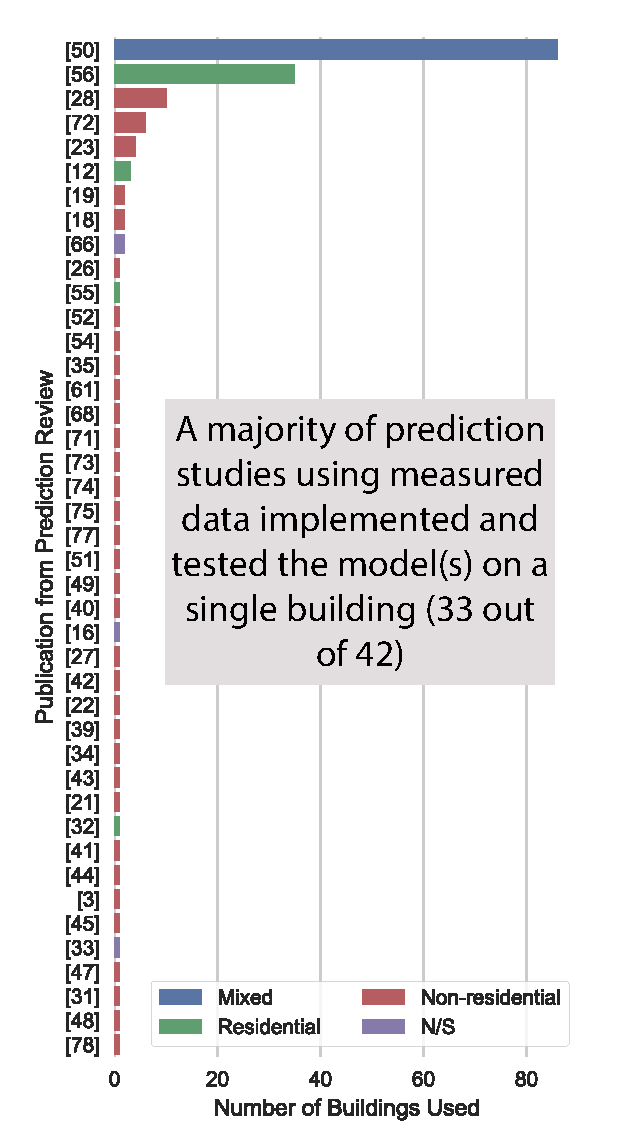
\includegraphics[width=0.4\columnwidth]{figures/numberofbuildings_annotated.pdf}
\caption{In the most recent prediction review study \cite{Amasyali2018AStudies}, a majority of publications developed and tested a machine learning modeling framework on data from a single building. These studies have the tendency to create very complex models for those particular buildings}
\label{fig:numberofsamples}%
\end{center}
\end{figure}

The results of the studies with a low number of samples are problematic from a machine learning standpoint as the techniques are mostly applied to a single building or a small set of buildings. Training a machine learning model on such a small set of data results in a solution that is grossly over-fitted for a specific scenario. Such over-fitting results in models that are inappropriate to apply to data from the wider building stock. Over-fitting is a well-understood challenge in the machine learning community. This concept is related the bias-variance trade off that is illustrated in Figure \ref{fig:bias-variance}. A model with high bias suffers from a lack of complexity to capture the behavior that is occurring in reality in a meaningful way. This model would be considered \emph{underfitting} the data. On the other hand, a model that is overly complex suffers from high variance; this model is able to capture all the detailed behavior in the data that is used to train the model, but the model does not perform as well with new data sets or future data.

\begin{figure}[ht!]
\begin{center}
\includegraphics[width=1\columnwidth]{figures/bias-variance-tradeoff.png}
\caption{Bias-variance trade-off - The graph shows how as complexity increases the \emph{bias} of the model drops as does the error rate. At a certain point the model becomes so complex that variance, or over-fitting becomes the key issue and the error rates increase again. The tree-based models below the chart show the increasing complexity of models of that type. Graphic adapted with permission from \cite{YeeStephanieModelTradeoff}}
\label{fig:bias-variance}%
\end{center}
\end{figure}

Three key studies were completed in the last four years which finally took the process of machine learning for prediction to a diverse set of buildings to attempt to tackle the issue of overfitting. The first used 400 randomly selected buildings and applied six common, open prediction models for the purpose of creating a measurement and verification baseline \cite{Granderson2015AutomatedModels}. The next study used 537 buildings and applied ten prediction models to further understand which model performed best among a large set of building \cite{Granderson2016AccuracyBuildings}. The final study focused on the evaluation of what percentage of the building stock are appropriate to be used with \emph{automated methods} as developed in the previous two studies \cite{Grandersona2017ApplicationData}. 

Overall, these studies tested a large set energy prediction methods on a large set of buildings and this method was a step in the direction of generalizability of energy prediction models. However, these studies are problematic due to the lack of access to the exact models or data the researchers used. Access to these aspects of their studies would allow future techniques to be compared directly through application of the old machine learning methods on new data or application of new machine learning methods on their old data. These studies give the community an understanding of what models work better than others in the context of the bias-variance trade-off, but they do not provide the ability to test new models and techniques.

\subsection{The importance of benchmarking - A remedy for a crisis of over-fitting}

Despite the advancement of machine learning and prediction for performance data for buildings, a major barrier to wide-spread dissemination is that the techniques are not easily reproducible and the results are not generalizable. Engineers, data scientists and researchers should be really asking themselves \emph{does my machine learning technique actually scale across hundreds of buildings? And is it actually faster or more accurate? How do we actually compare, each individual technique against previously created methods?}

The time-series data mining community identified this problem as early as 2003: ``Much of this work has very little utility because the contribution made''...``offer an amount of improvement that would have been completely dwarfed by the variance that would have been observed by testing on many real world data sets, or the variance that would have been observed by changing minor (unstated) implementation details. \cite{Keogh2003}'' This research group has most recently completed a large review of time-series classification algorithms on the UC Riverside open time-series data set \cite{Bagnall2017TheAdvances, UCRArchive}.

Since then, a large portion of the machine learning community has created a program called \emph{MLPerf} that uses benchmark data sets to test the software, hardware, and cloud-based solutions for applications such as image classification, speech recognition, sentiment analysis, and several other common machine learning challenges\footnote{https://mlperf.org/}. This effort is predicted to move the entire community forward by allowing for quantitative comparison of the library of techniques in the community. Several other good examples of benchmarking data set and analysis can be found in specific scientific domains such as biology \cite{Sonego2007ALearning}, information retrieval \cite{Liu2007LETORRetrieval}, and intrusion detection \cite{Kayack2005AnalysisAlgorithms}.

The built environment still struggles with over-fitting despite these advancements in the larger ML community. Figure \ref{fig:oldway} illustrates the conventional way that machine learning is generally implemented in the built environment domain. Most of the existing building performance data science studies rely on each individual researcher creating their own methods, finding a case study data set and determining efficacy on their own. Not surprisingly, most of those researcher find positive results. However, the ability to compare those results to other publications and techniques is limited. 

\begin{figure}[ht!]
\begin{center}
\includegraphics[width=1\columnwidth]{figures/Oldway}
\caption{Old anecdotal machine learning testing and implementation methodology that results in a lack of comparative opportunities for new techniques}
\label{fig:oldway}%
\end{center}
\end{figure}

Using a large, consistent benchmark data set from hundreds (or thousands) of buildings, a researcher can determine how well their methods actually perform across a heterogeneous data set. If multiple researcher use the same data set, then there can be meaningful comparisons of accuracy, speed and ease-of-use. The purpose of this paper is to establish an example of machine learning benchmarking for the purposes of energy forecasting and prediction.

\begin{figure}[ht!]
\begin{center}
\includegraphics[width=1\columnwidth]{figures/NewWay}
\caption{Using a common bench-marking data set enables the comparison of algorithms developed in the research community}
\label{fig:newway}%
\end{center}
\end{figure}

The creation of benchmarking data sets and methods sets the research community towards an environment in which there is a measure of accountability in the claims made by new algorithms. These new techniques will likely be implemented on the test case(s) developed in the course of a research study, but will need to also be applied as much as possible to benchmarking methods in order to show which type of improvement is occurring in the literature and the quantification of improvement. 

\subsubsection{A good example from the past - Great Energy Predictor Shootout I and II}

In the non-residential building research domain, there is a single set of examples of a benchmarking data set that was utilized for several machine learning studies. This set is the \emph{Great Energy Predictor Shootout} competitions held in the early 1990's. The first competition included the use of a single building's electrical, cooling, and heating meters in a competition where the participants were asked predict a single month of data using three months of training data \cite{osti_33315}. This competition resulted in several publication based on the top set of performers in the competition. A second competition was held, the aptly-named \emph{Great Energy Predictor Shootout II} that asked participants to predict the energy savings for a energy savings project \cite{haberl1996great}. These data sets have been since been used as a benchmarking comparison data set on two studies; one focused on residential modelling using SVM \ref{Gonzalez2005PredictionNetwork} and the other to predict consumption of office buildings in Greece \ref{Karatasou2006ModelingResults}.

\subsection{Tackling the over-fitting problem - open benchmarking data sets and open models}
\label{sec:outline}

This paper outlines a demonstration of how benchmarking of performance prediction models can be accomplished on an open data set using open-source prediction techniques. Initially in Section \ref{sec:modelling_considerations}, a review of prediction considerations for building energy performance is reviewed. Next, in Section \ref{sec:frameworkforanalysis} a framework for implementation is outlined using the Building Data Genome Project data set . In Section \ref{sec:results}, the results are showcased and interpreted in the context of the different primary use types and operations considerations. Finally, in Section \ref{sec:conclusion}, a discussion of the limitations and guidelines for implementation of future techniques is presented.
% \subsection{Previous literature on energy prediction for energy forecasting}
% \label{sec:litreview}
 
% An extensive review of performance prediction illustrates the diversity of algorithms and data types predicted in the last ten years \citep{Amasyali2018AStudies}. 
\section{Review of building energy prediction input considerations}
\label{sec:modelling_considerations}

To initiate the prediction model discussion, an overview of the conventional energy performance prediction considerations is covered in this section. These aspects of machine learning-based modelling for buildings are most prominent in non-residential buildings such as offices, educational facilities, laboratories, and health-care. These categories are the key considerations when developing prediction models for buildings.

\subsection{Daily, weekly and seasonal schedules}
\label{sec:schedules}
Buildings operate on several types of schedules. A majority of non-residential building have \emph{occupied} and \emph{unoccupied} periods that usually coincide with daytime and nighttime. These diurnal cycles are generally one of the best indicators of the building use type - i.e.: offices are open from 9am to 6pm and hotels are most active from 6pm to 10am. An example of daily pattern extraction and analysis is found in the \emph{DayFilter} process \cite{Miller2015AutomatedData}. Most buildings also have a weekly schedule; the default being certain behavior on weekdays and a different behavior on weekends. Finally, many buildings have seasonal changes such as when educational buildings have certain behavior during a regular session versus during breaks or holiday seasons. Extraction and analysis of longer term schedules is covered extensively in an overview of temporal feature extraction from meter data using the STL package \cite{Miller2017MiningBuildings,Cleveland1990STL:Statistics}. The concept of scheduling in non-residential building is most often related to the predefined schedules programmed into the automation systems in the building, unlike the human behavior that is discussed later. These schedules are determined usually by the operations and maintenance policy or by the energy management group within an organization. Many buildings have very predictable schedules, while others are much more volatile. Modelling such behavior can often be done using time-series methods that find auto-correlation behavior or by using date/time features as inputs to prediction models.

\subsection{Human behavior}
\label{sec:human}
The concept of \emph{human behavior} as an influence is similar to the previously-discussed schedules, however there is a more stochastic element to these behavior. Buildings that are more influenced by occupant behavior generally have demand response-based control systems that use sensors, cameras or other detection methods to modulate systems only when humans are present or using the space for a specific purpose \cite{Hong2018OccupantPrograms}. Sometimes humans even have the ability to control spaces using various types of interfaces with the building, although this is less common in non-residential buildings. Modelling occupant behavior is considered more complex than schedule as human behavior can be less systematic, thus auto correlation-based time-series methods are less effective. 

\subsection{Weather}
\label{sec:weather}
A major energy consuming component for most buildings are heating, ventilation, and air-conditioning (HVAC) systems. Intuitively, these systems tend to use more energy as the outdoor conditions get hotter (in the case of cooling) or colder (in the case of heating). Often this relationship is linear, but it can also be non-linear based on the HVAC system type and operation policy. Two common building performance modeling techniques address the influence of weather using \emph{change point models} \cite{KellyKissock2008MeasuringSavings} and the \emph{time-of-week and temperature} \cite{Mathieu2011QuantifyingResponse}. The degree of influence of weather varies greatly among the building stock. It is influenced by the percentage of internal load vs. envelope-based load, HVAC system type, climate, and other factors. 

\subsection{Non-routine events}
\label{sec:nre}
Non-routine events are disruptions in the systematic operation of a building due to events such as a change in the operational schedule of the building, equipment breakdowns, and events or human behavior that is highly irregular as compared to past behavior. These events could be planned or unplanned by the operations and facilities management staff. Non-routine events are hard to predict with conventional input variables, but models can be tuned to quickly adapt to the change using approaches related to change-point prediction or other types of behavior change detection techniques. Change point detection models are often unsupervised and some techniques have been adapted from the analysis of social media data to be used on energy meter data \cite{Miller2017MiningBuildings, James2016LeveragingBad}.

% \subsubsection{Energy conservation measures}
% \label{sec:ecm}

\section{Benchmarking open source prediction methods on open building energy data}
\label{sec:frameworkforanalysis}

\begin{figure}[ht!]
\begin{center}
\includegraphics[width=1\columnwidth]{figures/allbars.pdf}
\caption{Meta-data breakdown of the \emph{Building Data Genome Project} benchmarking data set used in this publication. Used with permission from \cite{Miller2017a}}
\label{fig:bdg_meta}%
\end{center}
\end{figure}


The key to this benchmarking analysis is to use a diverse enough data set to illustrate the benefits of scalabiliy and generalizabiliy amongst the building stock. The regression testing framework for this paper is outlined in this section. The open hourly data from the Building Data Genome Project is used in this paper as a starting point. This data set includes data from over 500 buildings, mostly from educational institutions. Figure \ref{fig:bdg_meta} illustrates the breakdown of four meta-data points from this data-set.

\subsection{Machine learning input variables}
\label{sec:variables}
The input variables available as independent predictors of energy consumption are outlined in this section. Table \ref{table:inputs} outlines the basic set of machine learning input variables used in this benchmarking approach. 

\begin{table}[h!]
\caption{Independent input features used in this benchmarking process}

\centering
\begin{tabular}{||c c c||} 
 \hline
 Category & Variable & Behavior Targeted \\ [0.5ex] 
 \hline\hline
 Temporal & Time of Day & Daily schedules \\ 
  & Day of Week  & Weekly schedules \\
  & Public Holiday Schedule & Holidays \\
  & Schedule Type & Seasonal schedules (summer, etc.) \\
 Weather & Outdoor Air Temp. & Sensible heating and cooling \\ 
  & Outdoor Air Hum. & Latent heating and cooling \\ 
%   & Outdoor Solar Rad.. & Cooling due to the sun \\ 
 Meta & Industry Sector & General category of use \\ 
  & Primary Use Type & Specific category of use\\ 
  & Floor area & Size of building\\ 
  & Number of floors & Height of building\\ 
  & Climate zone & Type of climate\\ 
  & Maximum occupancy & Total number of people\\ 
  & Cooling system type & Typical cooling efficiency\\ 
  & Heating system type & Typical heating efficiency\\
  & Performance rating & Comparison to its peers\\[1ex] 
 \hline
\end{tabular}
\label{table:inputs}
\end{table}

\subsection{Training and test data set scenario}
\label{sec:trainingandtesting}

For the purposes of the comparison of various open source techniques, a simplified training and testing scenario is utilized for the comparison. One year of whole building hourly electrical meter data is available for all 482 buildings. Four different training and testing data scenarios are tested as seen in Figure \ref{sec:trainingandtesting}. Scenarios 1-3 are made up of 3, 6, and 9 month training windows and a 3 month continuous testing window. Scenario 4 is made up of 3 month training windows followed by a 1 month test window that repeats itself three times. These scenarios provide a certain level of cross-validation that is realistic in the context of medium to long-term energy prediction in the built environment. 

\begin{figure}[ht!]
\begin{center}
\includegraphics[width=1\columnwidth]{figures/traing-testing.pdf}
\caption{Overview of the four training/testing scenarios}
\label{fig:training}%
\end{center}
\end{figure}

% These data is divided into 75\% test data and 25\% training data by removing every fourth month

\subsection{Open source regression models from Sci-kit Learn Python Library}
The regression model catalogue from the Sci-kit Learn Library is used in this benchmarking process. We use these models as a starting point for the benchmarking process as many of these models have been developed for decades and are some of the most often used prediction models in the machine learning community. The larger array of more advanced models (e.g.: deep learning, specific energy-focused prediction models) is left outside the scope of this paper as these will be the \emph{improved techniques} that the wider research community would likely be testing. 

This study focuses on general forecasting methods as a foundation for comparison for more building domain specific regression or prediction models. These models do not take into consideration the auto-correlation aspect of prediction or the building context-specific nature of the built environment. 



% \subsection{Open source time-series regression models from Statsmodel}
% The models from the Python package known as \emph{statsmodels} are applied.


% \subsection{Open source energy baseline models from M\&V 2.0}
% The models from the R package known as \emph{M\&V 2.0} are applied.

% \subsection{Open source energy baseline models from EEMeter}
% The models from the Python package known as \emph{EEMeter} are applied.

\subsection{Accuracy metrics}
The three metrics used in this analysis to evaluate model fit are the Normalized Mean Bias Error (NMBE), Coefficient of Variation of the Room Mean Square Error (CVRSME), and the Mean Absolute Percentage Error (MAPE). These metrics are all commonly used in the performance analysis of energy models in the building industry \cite{guideline2014guideline, organisation2007international}. The metrics are a combination of the values of number of compared values ($n$), measured values ($m$), predicted values ($f$), and parameters ($p$). Table \ref{table:metrics} illustrates the formulas for these metrics.

\begin{table}[h!]
\caption{Model performance metrics used in this benchmarking process}

\centering
\begin{tabular}{l r @{} >{${}}c<{{}$} @{} l}
\toprule
Coefficient of Variation of the Root \\Mean Squared Error & CV(RMSE) &= &$\displaystyle\frac{100\%}{\bar{m}}\sqrt{\frac{\sum_{i=1}^{n}(m_i-f_i)^2}{n-p}}$   \\
\midrule
Normalized Mean Bias Error & NMBE &= &$\displaystyle\frac{100\%}{\bar{m}}\frac{\sum_{i=1}^{n}(m_i-f_i)}{n-p}$   \\
 \\
\midrule
Mean absolute percentage error & MAPE &= &$\displaystyle\frac{100\%}{n}\sum_{i=1}^{n}\left |\frac{(m_i-f_i}{m_i}\right|$\\
\bottomrule
\end{tabular}
\label{table:metrics}
\end{table}

\section{Results}
\label{sec:results}

\subsection{Model fit overview}
\label{sec:accuracy}

Figure \ref{fig:model_fit} illustrates 12 Sci-Kit learn models applied to all the building use types using the MAPE and CVRSME metrics. The detailed results of all model implementations, including NBME, can be found in Appendix \ref{detailedmodels}. The graphics in the appendix provide a more detailed breakdown of each of the building use types according to all three error metrics as well as an analysis of each of the four training/testing scenarios. 

In general, laboratories have the highest accuracy across all of the models and in general. This situation is due to laboratories being the most \emph{systematically schedule-driven} of all the building types. Laboratories often have large equipment that is operated continuously or in set time schedules throughout the course of an entire year. University classrooms and offices behave in similar ways across the models as these two use types are often similar and many of these buildings are mixed use types. University dormitories have the fourth highest accuracy for most of the models, however they are better fits for models such as the Huber Regressor or the TheilSen Regressor. Finally, the Primary School buildings are the worst performers among the building use types. These buildings are dependent more on human behavior within their annual schedule phases, resulting in the lack of predictability using the methods and models outlined in this simple example.

\begin{figure}[ht!]
\begin{center}
\includegraphics[width=1\columnwidth]{figures/Cat_Plot.pdf}
\caption{Overview of models fit metrics MAPE and CVRSME for each building use type across 12 Sci-kit Learn models}
\label{fig:model_fit}%
\end{center}
\end{figure}

% \subsection{Error regions}
% \label{sec:error}
% This section shows the specific buildings that performed poorly using the prediction models and illustrates possible reasons why.

% They don't do such a good job of predicting buildings that are:

% The regions of mis-classification are

\section{Conclusion}
\label{sec:conclusion}
This publication gives readers a simple example of mainstream prediction techniques applied to a large, diverse data set. Five different primary use types of buildings were analyzed - offices, laboratories, university classrooms, dormitories, and primary/secondary schools. The mainstream models and input variables in this process produced reasonable results for most buildings with ensemble methods such as decision-tree based techniques such as ExtraTrees and Bagging regressors. Primary/Secondary schools stood apart as a difficult building type to predict due to seasonal shifts. 

% The results of this study This example is designed to illustrate how future techniques can and should be applied to open data sets.

\subsection{Limitations}
\label{sec:limitations}
The key limitation of this analysis is congruent with the limitation of machine learning in general: the models developed and the resulting metrics are limited by the range of training data utilized to build the models. The conclusions of the model comparison in this paper are only relevant to office, laboratories, classrooms, and dormitories from university campuses in the context of the geographical and operational environments of the Building Data Genome Project data set. Thus, the primary goal of this analysis is not to be comprehensive in capturing the behavior of the building stock, but to provide an example and data set that can be built upon with a more diverse set of data. \emph{It is crucial that additional data from thousands (or millions) of other buildings are added over time for the methodology to achieve the main goal of a comprehensive benchmarking process.}

New algorithms coming into the public domain should be tested against this growing set of building data sets to quantify what improvements are being made in the domain.

\subsection{Open Source Repository of Data and Implementation}
\label{sec:opensourcerepository}
This publication is fully reproducible using the code based from a Github respository focused on benchmarking for the built environment and data publicly available from the the Building Data Genome Project.

\subsection{Future work: the Great Building Energy Predictor Shootout 2019}
\label{sec:predictorshootout}
A machine learning competition is in the planning phase to further extend the benchmark data set to over 4000 energy data streams from 1200+ buildings from around the world. This competition will put potentially thousands of machine learning and building systems experts head-to-head to come up with the best set of methods to predict. 

Key areas of potential improvement include:
\begin{enumerate}
  \item Next generation time-series features - using the autocorrelated patterns of time-series data in more advanced ways
  \item Multi-variate learning - using a building's \emph{peers} to predict future behavior
  \item Advanced models - using deep learning to leverage new and diverse types of behavior without feature engineering
  \item Advanced ensembles - a voting ensemble that could significantly improve prediction for different building types
  \item White or Gray Box model convergence - using physics-based models to inform the machine learning algorithm
\end{enumerate}

% \appendix
% \section{Detailed Model Comparison Breakdowns}



\section{References}
\bibliographystyle{model1-num-names}
\bibliography{buildingenergyforecasting_mendeley}

%% Authors are advised to submit their bibtex database files. They are
%% requested to list a bibtex style file in the manuscript if they do
%% not want to use model1-num-names.bst.

%% References without bibTeX database:

% \begin{thebibliography}{00}

%% \bibitem must have the following form:
%%   \bibitem{key}...
%%

% \bibitem{}

% \end{thebibliography}

\appendix
\section{Detailed Model Comparison Breakdowns}
\label{detailedmodels}

\begin{figure}[ht!]
\begin{center}
\includegraphics[width=1\columnwidth]{figures/Office_boxplot.pdf}
\caption{Detailed Breakdown of Benchmarking Models on Office Buildings}
\label{fig:offices}%
\end{center}
\end{figure}

\begin{figure}[ht!]
\begin{center}
\includegraphics[width=1\columnwidth]{figures/UnivClass_boxplot.pdf}
\caption{Detailed Breakdown of Benchmarking Models on University Classroom Buildings}
\label{fig:class}%
\end{center}
\end{figure}

\begin{figure}[ht!]
\begin{center}
\includegraphics[width=1\columnwidth]{figures/UnivLab_boxplot.pdf}
\caption{Detailed Breakdown of Benchmarking Models on University Laboratory Buildings}
\label{fig:lab}%
\end{center}
\end{figure}

\begin{figure}[ht!]
\begin{center}
\includegraphics[width=1\columnwidth]{figures/UnivDorm_boxplot.pdf}
\caption{Detailed Breakdown of Benchmarking Models on University Dormitory Buildings}
\label{fig:dorms}%
\end{center}
\end{figure}

\begin{figure}[ht!]
\begin{center}
\includegraphics[width=1\columnwidth]{figures/PrimClass_boxplot.pdf}
\caption{Detailed Breakdown of Benchmarking Models on Primary School Buildings}
\label{fig:prim}%
\end{center}
\end{figure}

\end{document}

%%
%% End of file `elsarticle-template-1-num.tex'.